\input{preamble}

%\newcommand{\xC}{\mathbb{C}}
\newcommand{\xR}{\mathbb{R}}
\newcommand{\xRd}{{\xR^d}}
\newcommand{\xRN}{{\xR^N}}
\newcommand{\xMNR}{{M_N(\xR)}}
\newcommand{\bb}{{\boldsymbol b}}
\newcommand{\ee}{{\boldsymbol e}}
\newcommand{\ev}{{\boldsymbol \epsilon}}
\newcommand{\rr}{{\boldsymbol r}}
\newcommand{\xx}{{\boldsymbol x}}
\newcommand{\hx}{\hat{\boldsymbol x}}
\newcommand{\yy}{{\boldsymbol y}}
\newcommand{\vv}{{\boldsymbol v}}
\newcommand{\ww}{{\boldsymbol w}}
\newcommand{\zz}{{\boldsymbol z}}
\renewcommand{\mA}{{\mathrm A}}
\newcommand{\mB}{{\mathrm B}}
\newcommand{\mC}{{\mathrm C}}
\newcommand{\mD}{{\mathrm D}}
\newcommand{\mG}{{\mathrm G}}
\newcommand{\mH}{{\mathrm H}}
\renewcommand{\mL}{{\mathrm L}}
\newcommand{\mLs}{{\mathrm L_0}}
\newcommand{\mM}{{\mathrm M}}
\newcommand{\mRs}{{\mathrm R_0}}
\newcommand{\mR}{{\mathrm R}}
\newcommand{\mP}{{\mathrm P}}
\newcommand{\mQ}{{\mathrm Q}}
\newcommand{\mU}{{\mathrm U}}
\newcommand{\mId}{{\mathbf{Id}}}
\newcommand{\mII}{{\mathbf{\mathbb{I}}}}
\newcommand{\Seq}[1]{\bigl(#1\bigr)}
\newcommand{\Cond}[1]{\mathcal{C}(#1)}
\newcommand{\Order}[1]{\mathcal{O}\left(#1\right)}
\newcommand{\norm}[1]{{\lVert #1 \rVert}}
\newcommand{\norminf}[1]{\norm{#1}_{\infty}}

\newcommand{\InnerK}[2]{{{\mathbf\langle}\;#1\:,\: #2 \;{\rangle}}}
\newcommand{\Inner}[2]{{{\scriptstyle\mathbf{(}}\;#1\:,\: #2 \;{\scriptstyle\mathbf{)}}}}


\newtheorem{ex}{Question}


\title{Review of previous examinations}
\institute{NTNU, IMF}
\date{April 20. 2018}
%\author{Based on 2016v slides by Eivind Fonn}
%\author{Aurélien Larcher}

\maketitle


\begin{frame}
  \frametitle{Examination}

The examination is usually comprised of:
\begin{itemize}
\item one problem related to linear algebra operations with calculation of complexity and parallelism.
\item one problem related to parallelization of solver for partial differential equations.
\item a series of short questions covering all the topics of the course.
\end{itemize}
to be solved in four hours.

\end{frame}
%-----------------------------------------------------------------------------

\begin{frame}
  \frametitle{Important points}

The course covered a broad range of topics, but a few points are important:
\begin{itemize}
\item Differentiate between the different types of parallelism (data, functional/task, and fine-/coarse-grained).
\item Be able to categorize hardware architectures, e.g with Flynn's taxonomy and understand their benefits/drawbacks.
\item Understand the memory hierarchy of computers and how it affects the performance of solvers.
\item Be able to define clearly and use the distributed and the shared-memory model.
\item Have a basic knowledge of the different specifications (OpenMP, MPI, BLAS) and libraries (LAPACK, PETSc) discussed. 
\end{itemize}

\end{frame}
%-----------------------------------------------------------------------------


\begin{frame}
  \frametitle{Notions used in Problems}

Study of parallel performance of algorithms.

\medskip
\textbf{Amdahl's law}: speed-up on $p$ processor w.r.t serial
\begin{equation*}
\mathcal{S}_p = \dfrac{T_1}{T_p} = \dfrac{p}{f (p - 1) + 1}
\end{equation*}
with $f$ fraction of time spent in serial sections of the code.

\medskip
The fraction $f$:
\begin{itemize}
\item $\rightarrow 1$ for purely serial case\\[2ex]
\item $\rightarrow 0$ for ideal parallel case
\end{itemize}

Linear strong scaling: $f = 0$
\begin{equation*}
S_p = \dfrac{T_1}{T_p} = p
\end{equation*}
ideal speed-up when solving a fixed problem on $p$ processors.

\end{frame}
%-----------------------------------------------------------------------------

\begin{frame}
  \frametitle{Notions used in Problems}
Some notions are important and will be used during the examination.

\medskip
Linear model for transmission:
\begin{equation}
\tau_c(k) = \tau_s + \gamma k
\end{equation}
with $\tau_s$ a constant that is the start-up phase and $\gamma$ the inverse bandwith.

\textbf{Amdahl's law}: speed-up on $p$ processor w.r.t serial
\begin{equation*}
\mathcal{S}_p = \dfrac{p}{p\dfrac{T_c}{T_1} + 1}
\end{equation*}
with $T_c$ the time spent in communications, a function of $\tau_c$.


\end{frame}

%----------------------------------------
\begin{frame}
  \frametitle{Challenges of parallel computing}


\begin{figure}
  \centering
  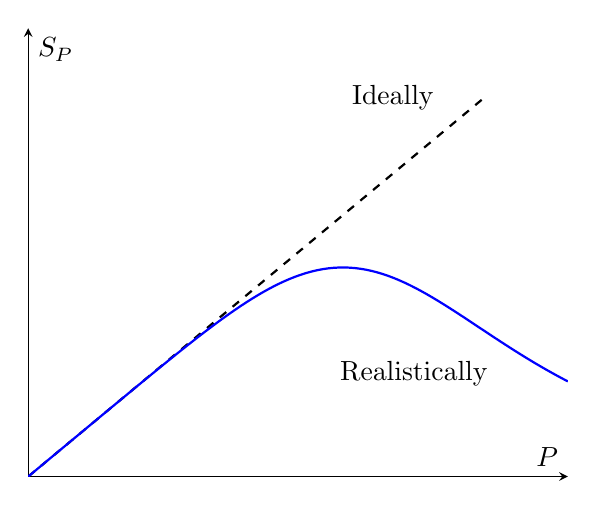
\begin{tikzpicture}
    \begin{axis}[
      xmin=0,
      xmax=1.3,
      ymin=0,
      ymax=1.3,
      axis lines=middle,
      ticks=none,
      xlabel={$P$},
      ylabel={$S_P$},
      ]
      \addplot[dashed, thick, domain=0:1.1, samples=100]{x};
      \addplot[blue, thick, domain=0:1.3, samples=100]{x/(1+x^5)};
      \node at (axis cs:1.0,1.1) [anchor=east] {Ideally};
      \node at (axis cs:1.13,0.3) [anchor=east] {Realistically};
    \end{axis}
  \end{tikzpicture}
  \caption{Ideal speedup ($S_P = P$) and realistic speedup.}
  \label{fig:scalability}
\end{figure}

\medskip
$\rightarrow$ strong scaling should be interpreted carefully!\\
$\rightarrow$ weak scaling should also be considered.

\end{frame}
%-----------------------------------------------------------------------------

\begin{frame}[fragile]
  \frametitle{Questions: Parallel computing}

\begin{ex}[2016]
A good strategy for reducing communication overhead is to increase the
number of processes. Answer: true or false
\end{ex}

It is crucial to remember Amdhal's Law, and for instance the practical effect observed in your project when studying the strong scaling.

\begin{ex}[2015]
A code with a large parallel efficiency typically has much network traffic.
\end{ex}

The same arguments apply.

\begin{ex}[2015]
A code with a large parallel speedup has a large parallel effciency.
\end{ex}

The same arguments apply.

\end{frame}
%-----------------------------------------------------------------------------

\begin{frame}[fragile]
  \frametitle{Questions: Computer architecture}

\begin{ex}[2016]
The following loops are compiled with an optimizing compiler:
\begin{itemize}
\item  Which of them will likely have the highest performance (more FLOPS)?
\item The following loops are compiled with an optimizing compiler. Which of
them will likely have the highest performance (more FLOPS)? 
\end{itemize}
Answer: A, B or none. Briefly explain why.
\end{ex}

A:
\begin{lstlisting}[style=c]
for (int i = 0; i < N ; i ++)
   a[i] = a[i] + b [i];
\end{lstlisting}
B:
\begin{lstlisting}[style=c]
for (int i = 0; i < N ; i ++)
   a[i] = a[i] + c * b [ i ];
\end{lstlisting}

Remember the definition of FLOPS and the capabilities of processor when it comes to floating-point operations.
\end{frame}
%-----------------------------------------------------------------------------

\begin{frame}[fragile]
  \frametitle{Questions: Computer architecture}

\begin{ex}[2015]
A ccNUMA machine can always do multiple additions in parallel. Answer: true or false
\end{ex}

Remember Flynn's taxonomy and the discussion on different computer architectures.

\begin{ex}[2015]
An LFU cache replacement policy is typically the best for solving partial
differential equations
\end{ex}

The question was briefly discuss in the description of different caching policies: First-In First-Out (FIFO), Least-Frequent Used (LFU), Least-Recently Used (LRU) and the pseudo-LRU.
Even without remembering the details of the implementation, you can think about the memory access pattern.

\end{frame}
%-----------------------------------------------------------------------------
\begin{frame}[fragile]
  \frametitle{Questions: Computer architecture}

\begin{ex}[2015]
A SIMD processor can perform a multiplication and an addition simultanously. Answer: true or false.
\end{ex}

Remember Flynn's taxonomy to motivate your answer.

\begin{ex}[2015]
Cancellation is a concern when subtracting floating point numbers. Answer: true or false.
\end{ex}

Remember the binary representation of floating-point numbers and how it affects the decimal precision.

\begin{ex}[2014]
Floating point numbers of a given precision can only represent a fixed range
of numbers.
\end{ex}

Remember the binary representation of floating-point numbers.

\end{frame}
%-----------------------------------------------------------------------------

\begin{frame}[fragile]
  \frametitle{Questions: Computer architecture}

\begin{ex}[2014]
A modern processor typically has a cache hierarchy. These are designed as
levels, where a higher level is given to faster memory.
\end{ex}

Remember for instance the architecture of modern CPUs and the different memory levels. 

\begin{ex}[2014]
A superscalar processor can perform two additions simultanously.
\end{ex}

Remember the discussion about pipelining.

\end{frame}
%-----------------------------------------------------------------------------

\begin{frame}[fragile]
  \frametitle{Questions: Distributed memory}

\begin{ex}[2016]
\begin{itemize}
\item It is always OK to call MPI library functions from different threads. Answer:
true or false.
\item It is never OK to call MPI library functions from different threads. Answer:
true or false.
\end{itemize}
\end{ex}

{\scriptsize
\begin{lstlisting}[style=c]
MPI_THREAD_SINGLE
    Only one thread will execute. 
MPI_THREAD_FUNNELED
    The process may be multi-threaded, but only the main thread will
    make MPI calls (all MPI calls are funneled to the main thread). 
MPI_THREAD_SERIALIZED
    The process may be multi-threaded, and multiple threads may make MPI calls, but only one at a time: MPI calls are not made concurrently from two distinct threads (all MPI calls are serialized). 
MPI_THREAD_MULTIPLE
    Multiple threads may call MPI, with no restrictions. 
\end{lstlisting}
}

In practice \texttt{MPI\_THREAD\_SINGLE} only is portable, see Balaji (2010) for a discussion.

\end{frame}
%-----------------------------------------------------------------------------

\begin{frame}[fragile]
  \frametitle{Questions: Distributed memory}

\begin{ex}[2011]
Consider the MPI-function below: the amount of data sent corresponds to 128 floating point numbers in double precision.
Answer: true or false.
\end{ex}

{\scriptsize
\begin{lstlisting}[style=c]
MPI_Send(buffer, 1024, MPI_DOUBLE, dest, tag, MPI_COMM_WORLD);
\end{lstlisting}
}

Writing the code for the projects should make this question easy.

\begin{ex}[2011]
The most efficient implementation of the \texttt{MPI\_Allreduce} operation on P processors
completes in a certain number of communication stages. Which of the 4 alternatives is correct: (i) 1 stage; (ii) log 2 (P ) stages; (iii) 2 log 2 (P ) stages; (iv) P stages
\end{ex}

Remember your implementation in Project I.

\end{frame}
%-----------------------------------------------------------------------------

\begin{frame}[fragile]
  \frametitle{Questions: Distributed memory}

\begin{ex}[2011]
The functions \texttt{MPI\_Send} and \texttt{MPI\_Recv} are appropriate to use for the exchange of an interprocess boundary. Is it possible to experience "deadlock" when using these functions? Answer: yes or no.
\end{ex}

Knowledge of point-to-point communication is sufficient.


\end{frame}
%-----------------------------------------------------------------------------

\begin{frame}[fragile]
  \frametitle{Questions: Shared-memory model}


\begin{ex}[2016]
Since threads do not need to communicate (like processes do), there is no
penalty incurred by using more of them. Answer: true or false.
\end{ex}

Remember how OpenMP works and the difference between concurrency and parallelism.

\begin{ex}[2014]
OpenMP is usable from all programming languages.
\end{ex}

Just enough to know about the OpenMP specification.

\end{frame}
%-----------------------------------------------------------------------------

\begin{frame}[fragile]
  \frametitle{Questions: Numerical Linear Algebra}


\begin{ex}[2016]
BLAS is a high performance library for solving linear systems of equations.
Answer: true or false.
\end{ex}

Remember how the specification was introduced during the lecture.
Hint: different level of algebric operations.

\begin{ex}[2015]
In code utilizing dense linear algebra, you have to choose between using
BLAS or LAPACK. Answer: true or false.
\end{ex}

Similar question, the relation betweeen BLAS and LAPACK is important to remember.

\end{frame}
%-----------------------------------------------------------------------------

\begin{frame}[fragile]
  \frametitle{Questions: Numerical Linear Algebra}

\begin{ex}[2015]
Using PETSc there is no point in pre-declaring the sparsity pattern of your
operator. Answer: true or false.
\end{ex}

Review how the storage for a sparse matrix is handled and how it may affect the performance.

\begin{ex}[2014]
You typically get performance closer to the theoretical peak performance of
a machine when you do level 1 operations (vector operations) compared to
level 3 (matrix-matrix operations).
\end{ex}

Think about the ratio between operations and data movement.

\end{frame}
%-----------------------------------------------------------------------------

\begin{frame}[fragile]
  \frametitle{Questions: Parallel Input/Output}

\begin{ex}[2015]
MPI-I/O is often used to do post-mortem data assembly.
Answer: true or false.
\end{ex}

The exact term as not been mentioned during the lecture but remember how the MPI-I/O implementation works.

\begin{ex}[2014]
MPI-I/O always writes multi-dimensional arrays in Fortran order.
\end{ex}

Just remember the purpose of MPI-I/O.

\end{frame}
%-----------------------------------------------------------------------------

\input{postamble}
